%!TEX root = ../main.tex
\subsection{System Requirements} % (fold)
\label{sec:system_requirements}
\begin{table}[H]
\centering
\caption{System requirements}
\label{tab:requirements}

\begin{tabular}{ |p{0.3cm}|p{10.5cm}| }
\hline
\multicolumn{2}{|c|}{\textbf{Functional}}\\
\hline
1 & Read data from sensors/data producers 				\\
2 & Timestamps all data 								\\
3 & Transmit data wireless between Zybo and monitoring station	\\
4 & Log data to SD card 								\\
5 & Transfer logs to monitoring station 								\\
6 & Start/stop transmission from nodes 					\\
7 & Present data to user								\\
8 & Provide an API for data access						\\
9 & Must continue to function on node failure			\\

\hline
\multicolumn{2}{|c|}{\textbf{Operational}}\\
\hline	
10 & A developer can add new nodes 										 \\
11 & A developer can modify existing nodes 								 \\
12 & A user can start/stop data transmission from nodes					 \\
13 & A user can request a data log 										 \\
14 & A developer can add API for specific sensor 						 \\
15 & A developer can add custum (G)UI									 \\


\hline
\multicolumn{2}{|c|}{\textbf{Quality of Service}}\\
\hline	
16 & Can support 16 nodes							 					\\
17 & Has wireless range of > 80 m						 				\\
18 & CAN network has 1 Mb/s data bandwidth			 					\\
19 & Timestamps with a precision of 1 ms 			 					\\

\hline
\multicolumn{2}{|c|}{\textbf{Design}}\\
\hline	
20 & Must allow for integration of new nodes		 					 \\
21 & Software must be modular to allow for simple integration of nodes	 \\

\hline
\multicolumn{2}{|c|}{\textbf{Interfaces}}\\
\hline	
22 & USB 		 						\\
23 & 5 V DC		 						\\
24 & WiFi	 							\\
25 & CAN 		 						\\
26 & CANOpen 		 					\\
27 & SD-card 		 					\\
\hline
\end{tabular}
\end{table}

\newpage
\begin{figure}[!h]
	\centering
	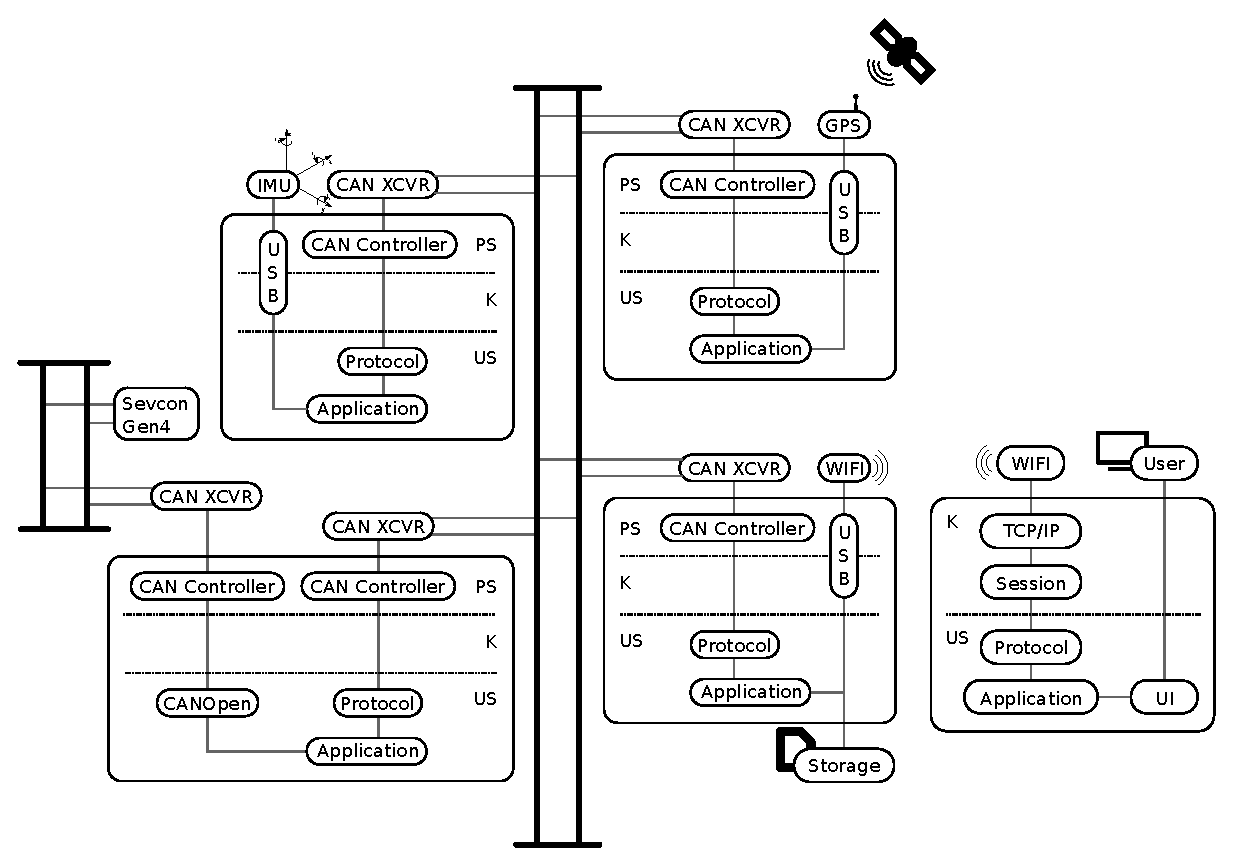
\includegraphics[angle=90,width=\textwidth]{graphics/analysis_complex.eps}
	\caption{An overview of the entire system to be implemented. The four nodes are depicted with their PS level, kernel and User Space. Two CAN busses are displayed by bold, parallel lines.}
	\label{fig:complete_system}
\end{figure}

% \subsection{Actors}
% The only actor on the system is an engineer.

% \subsection{Interfaces}
% \begin{itemize}
% \item Wifi, for data transfer between go-kart and stationary computer.
% \item CAN bus, for local network.
% \item CanOpen, for interfacing the Sevcon.
% \item USB, for GPS and IMU.
% \item ??, for SD card connection.
% \item Powersupply, for Zybos.
% \end{itemize}

% \subsection{Functional requirements}
% The system: 
% \begin{itemize}
% \item Reads data from sensors.
% \item Reads data from Sevcon.
% \item Transfers data to stationary computer using Wifi.
% \item Presents data to the user.
% \item Logs sensordata to SD card.
% \item Read data from SD card.
% \item Timestamps all data. 
% \end{itemize}

% \subsection{Operational requirements}
% The system monitors go-kart data.% when engineer starts the system by powering it on.

% \subsection{Quality of service requirements}
% \begin{itemize}
% \item IMU data must be sampled with xx Hz.
% \item GPS data must be sampled with zz Hz.
% \item Data logging with qq Hz.??
% \end{itemize}

% \subsection{Parametric requirements}
% Wifi range must be greater than xx meters.

% \subsection{Design requirements}
% The system:
% \begin{itemize}
% \item must be scalable to at least 16 sensors/nodes.
% \item must be modular to allow easy integration of new sensors/nodes.
% \item must be functional if one or more sensors/nodes stop working.	 
% \end{itemize}


% section system_requirements (end)